\documentclass[a4paper,12pt]{article}
\usepackage[utf8]{inputenc}
\usepackage{algorithmic}
\usepackage{algorithm}
\usepackage{pst-plot}
\usepackage{graphicx}
\usepackage{endnotes}
\usepackage{graphics}
\usepackage{graphicx}
\usepackage{floatflt}
\usepackage{wrapfig}
\usepackage{amsfonts}
\usepackage{amsmath}
\usepackage{verbatim}
\usepackage{hyperref}
\usepackage{multirow}
\usepackage{pdflscape}
\usepackage{multicol}
\usepackage[bottom]{footmisc}

\usepackage{hyperref}
\hypersetup{pdfborder={0 0 0 0}}

\pdfpagewidth 210mm
\pdfpageheight 297mm 
\setlength\topmargin{0mm}
\setlength\headheight{0mm}
\setlength\headsep{0mm}
\setlength\textheight{250mm}	
\setlength\textwidth{159.2mm}
\setlength\oddsidemargin{0mm}
\setlength\evensidemargin{0mm}
\setlength\parindent{0mm}
\setlength\parskip{3mm}

\graphicspath{{./images/}}



%
% Title
%
\begin{document}
\begin{center}
	{\Large
	University of Tartu\\
	Faculty of Mathematics and Computer Science\\
	Institute of Computer Science\\}
	\vspace{6cm}
	{\Large Kristjan Korjus, Ilya Kuzovkin, Ardi Tampuu, Taivo Pungas}\\
	\vspace{1.0cm}
	{\Huge Replicating the Paper ``Playing Atari with Deep Reinforcement Learning"\textsuperscript{\Large{\cite{mnih2013playing}}}}\\
	\vspace{0.5cm}
	{\Large Technical Report}\\
	\vspace{1.0cm}
	{\large MTAT.03.291 Introduction to Computational Neuroscience}
	
\end{center}
\vspace{9cm}
\begin{center}
	{\large Tartu 2014}
\end{center}
\thispagestyle{empty}
\pagebreak



%
% Table of contents
%
\thispagestyle{empty}
\tableofcontents
\pagebreak



%
% Introduction
%
\section*{Introduction}
\addcontentsline{toc}{section}{Introduction}
In the recent years the popularity of the method called \emph{deep learning}\textsuperscript{\cite{hinton2007learning}} has increased noticeably in the machine learning community. Deep leaning was successfully applied to speech recognition\textsuperscript{\cite{dahl2012context}} and many other tasks in machine learning\textsuperscript{\cite{deng2013new}}. In all these studies the performance of the resulting system was better than other machine learning methods were able to achieve so far.

The core of the deep learning method is an artificial neural network. One of the properties, which gives this family of learning algorithms a special place, is the ability to extract a ``meaningful" (from the human perspective) \emph{concepts} from the data by combining the features based on the structure of the data. The extracted concepts sometimes have clear interpretation and that makes us feel as if the machine has indeed \emph{learned} something. Here we step into the realm of artificial intelligence, the possibility of which never stops to fascinate our minds.

One of the recent works, which brings together deep learning and artificial intelligence is a paper ``Playing Atari with Deep Reinforcement Learning"\textsuperscript{\cite{mnih2013playing}} published by DeepMind\footnote{\url{http://deepmind.com}} company. The paper describes a system, which combines deep learning methods and the \emph{reinforcement learning} in order to create a system that is able to learn how to play simple computer games. It is worth mentioning that the system has access only to the visual information (screen of the game) and the scores. Based on these two inputs the system learns to understand which moves are good and which are bad depending on the situation on the screen. Notice that the human player uses exactly same information to evaluate his performance and adapt his playing strategy. The reported result shows that the system was able to master several different games and play some of them better than the human player.

This result can be seen as a step forward to the truly intelligent machines and thus it fascinates us. The goal of this project is to create an open-source analogue of such a system using the description provided in the paper.



%
% Bird-eye view
%
\pagebreak
\section{Overview of the system}
Before we go into the details, let us describe the overall architecture of the system and show how the building blocks are put together. 

\subsection{The task}

The system receives a picture of a game screen (an example is shown in Figure \ref{fig:breakoutscreen}) and chooses an action to take. It then executes this action and is told whether the score increased, decreased or did not change. Based on this information and playing a large number of games, the system needs to learn to improve its performance in the game.

\begin{figure}[h]
\centering
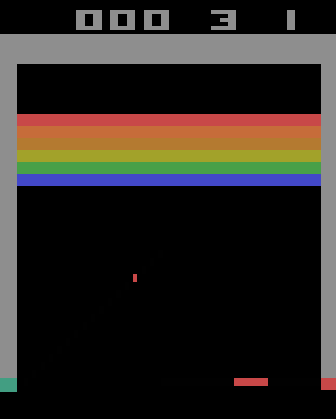
\includegraphics[width=3.5cm]{fig_gamescreen}
\caption{A game screen of Breakout.}
\label{fig:breakoutscreen}
\end{figure}

\subsection{Reinforcement learning}
In a reinforcement learning setting, an agent takes actions in an environment with the goal of maximising a cumulative reward. We tried to create a software agent that plays ATARI games in an emulator (the environment) and maximises its performance in the game, measured by its score in the games.

\subsubsection{Exploration-exploitation}
When the algorithm chooses between possible actions, it picks a ``learned" action with probability $1-\epsilon$ and a random action with probability $\epsilon$. The value of $\epsilon$ is gradually decreased as the algorithm learns to play better.

It is necessary to sometimes pick a random action to not get stuck in local reward maxima. At first, the value of $\epsilon$ is small and the agent takes random actions most of the time. This relatively high emphasis on exploration is necessary for the agent to collect information about the environment. When $\epsilon$ starts to decrease, the agent starts to apply its learned behaviour more and more, i.e. moving towards exploitation.

$\epsilon$ never reaches zero in the case of our agent, so it still does some exploration even when performing well in the game.

\subsection{Neural network}
The system uses a neural network to assign an expected reward value to each possible action. The input to the network at any time point consists of the last four preprocessed game screens the system received. This input is then passed through three successive hidden layers to the output layer. 

The output layer has one node for each possible action and the activation of those nodes indicates the expected reward from each of the possible actions - here, the action with the highest expected reward is selected for execution.

\subsection{Learning process}
Under the fancy word ``neural network" hides a quite simple idea: bunch of \emph{nodes} (neurons), each of them having some \emph{input} to perform a computation on and an \emph{output} where the result of the computation will be sent to, are connected to each other. Each connection has a \emph{weight}, which regulates how much one neuron can affect another. The very first layer of the network is usually called the \emph{input layer}. This is the place where we inject a data sample. Next to the input layer the network has several trickily connected \emph{hidden layers}. And the last layer is an \emph{output layer}, it gives us the final piece of information we wanted to know about the data sample we fed into the network. The resulting structure can be very complex, but the building blocks are always the same: neurons and connections between them.

We, as the builders of the system, usually know what we want it do: that is for each data sample we know what the final output should look like. Now the ``smart" neural network is the one able to produce the output we expect, the ``naive" network is the one which is not. The only thing that differs in those two are the \emph{weights} on the connections between the nodes. By changing them in accordance with our final goal the network goes from being ``naive" to being ``smart". This process in general in known as \emph{learning}.

To explain the concept of learning to the machine we introduce the notion of \emph{cost function} (or \emph{loss function}) which we will denote by $L$. Given the parameters of the network this function goes over the data samples, computes the outputs, compares these outputs with the expected ones and calculates how big is the error the system makes. The learning process can be represented as the process of \emph{minimizing} the cost function.

The obvious way to minimize a function is to try out all possible inputs to find the minimal output. Unfortunately the number of possible input is unfeasibly large. How to do it is a big question not only for our system. The whole brach on computer science called \emph{optimization} is dealing with this issue. One of the most popular technique used in this area is called \emph{gradient descent}.

The idea of gradient descent is rather trivial: at each \emph{iteration} of the learning algorithm it makes a small step in the ``direction" which makes the value of the loss function smaller. Thus by making enough steps the algorithm will reach an \emph{optimum}: a place from where step in any direction will only increase the value of the loss function. Once this optimum is found we say that the learning has finished and the system is now as smart as it can be. It might happen that the optimum we found is not the best one (\emph{local optimum}), and there are bunch of techniques (for example \emph{Monte Carlo} methods) to find the \emph{global optimum}, but we will not dwell into this right now. 

Gradient descent uses the \emph{gradient} (multidimensional derivative) as it's core:
\begin{enumerate}
	\item Let the current configuration of the system be $\mathbf{w_0}$
	\item Compute the derivative (gradient) of the loss function at this point $L(\mathbf{w_0})$
	\item Look at the derivative with respect to each element $(w_1, \ldots, w_n) = \mathbf{w_0}$ and:
	\begin{enumerate}
		\item If the derivative is 0 then we should not touch this parameter of our system
		\item Otherwise move one step in the direction opposite to the derivative (positive slope -- decrease the parameter, negative slope -- increase the parameter)
	\end{enumerate}
	\item Repeat starting from the step 2. until the derivatives with respect to all parameters of the system are zeros (or close to zeros)
\end{enumerate}
Once this process is complete we believe that our system has reached the optimal state: it's parameters are configures in such way that it will give optimal performance on the dataset we have. In our system we will use variation of the idea of gradient descent called RMSProp, you will read about it later.



%
% Components
%
\section{Components of the system}
here goes the detailed description of everything (aka the hardest part)


\subsection{Launching and communicating with ALE}

Just as we, humans, exchange information with a computer game by seeing the computer screen (input) and pressing the keys (output actions), the system needs to communicate with the Arcade Learning Environment that hosts the game.
\paragraph{}
The communication with ALE is achieved using two first-in-first out pipes which must be created before the ALE is launched. We create the pipes and launch ALE using the os package of Python. The parameters given to ALE at execution must specify the way we want to communicate with ALE (FIFO pipes) and the location of the binary file containing the game to run (Breakout). In addition, we specify that we want ALE to return unencoded images, that only every 4th frame should be sent to us and whether the game window should be made visible.


\paragraph{}
The actual communication starts with a handshake phase, where we define the desired inputs (screen image and episode information) and ALE responds by informing us about the dimensions of the image. Thereafter the conversation between ALE and our agent consists in reading and deciphering inputs from FIFO\_in pipe and sending the chosen actions back through FIFO\_out pipe. The information is read from pipes as one long String, so deciphering is needed (cutting the input and converting the pieces into appropriate types). Similarly, the chosen action has to be transformed to an output string of specific format. If a game is lost, a specific "reset" signal is sent to start the next game. When the desired number of games has been played, the communication with ALE can be terminated by closing the communication pipes. 



\subsection{Convolutional neural network}
Our system receives 4x84x84 pixel values as input. In order to find relevant information from these four 84x84 images, we use convolutional neural networks (CNN) [reference???]. CNNs are a specific type of neural network that are particularly adapted to extract features from images.
\paragraph{}
Unlike RBMs which see their input as an 1D vector, a CNN treats the input images as 2D objects. These 2D matrices of pixel values are convolved with linear filters to obtain the activities of the next layer. For example, our first hidden layer is generated by convolving our images with sixteen different 8x8 filters, using a step of 4 pixels. This means that for each of the 16 different filters, we first take the topleft 8x8 values of an image and linearly combine them with the filter, obtaining as a result one activity value. We then move 4 pixels left and multiply another 8x8 area from the image with the same filter (same weight values). When reaching the right edge of the image, we start again from the left, only 4 pixels lower. Each linear combination yields one activity value, so convolving an 84x84 image with an 8x8 filter with step 4 produces 20x20 topologically arranged values. As we apply 16 different filters, we end up with 16*20*20 nodes in the first hidden layer of our convolutional network.
\paragraph{}
An attentive reader notices that our input consists of 4 images, not only one. This means that each of our filters contains four weight matrices of size 8x8. The images will be convolved with the corresponding 8x8 matrix and the calculated activities are summed up, so we end up with 16*20*20 values as before. All in all, $W^{KL}_{ij}$ denotes the weight value connecting the pixel value on coordinates (i,j) of the selected 8x8 area of the L-th image with the K-th feature map.

\paragraph{}
Last but not least, a linear rectifier is applied to the activity values, setting all negative values to 0.
\paragraph{}
The obtained sixteen 20x20 feature maps are thereafter convolved with 32 4x4 filters. Using a step of 2, this yields 32x9x9 activity values in the second hidden layer. As before, the filters are not 2-dimensional, instead they have 16x4x4 values.
\paragraph{}
With these two convolutional layers we have reduced the number of nodes from 4x84x84 to 32x9x9. Functionally, after training the system we expect the nodes of the second hidden layer to represent spatiotemporal patterns relevant for successfully playing the game.

\subsection{Q-learning}
...

\subsection{RMSProp}
...


\subsection{And once again how all those things are put together}



%
% Implementation
%
\pagebreak
\section{Implementation details}
Programming language: Python 2.7 (32-bit).

Python libraries used: Pillow, NumPy, Theano.

ATARI emulation environment: ALE (Arcade Learning Environement).

\subsection{Agent}
...

\subsection{Memory}
...

\subsection{Preprocessing}
\label{subsection_preproc}
The game screens are preprocessed by cropping the original 160x210-pixel image to a 160x160 region of interest, which is then downscaled to a 84x84 image.

The colors from ATARI's NTSC palette are converted to RGB using a conversion table
\footnote{\url{http://www.biglist.com/lists/stella/archives/200109/msg00285.html}}. The RGB representation is then converted to grayscale according to the weighted combination $0.21R + 0.71G + 0.07B$. This should produce a representation close to human perception (humans are more sensitive to green than other colours)\footnote{\url{http://www.johndcook.com/blog/2009/08/24/algorithms-convert-color-grayscale/
}}. An example of a preprocessed image is shown in Figure \ref{fig:breakoutpreprocessed}.

\begin{figure}[h]
\centering

\includegraphics[width=2.5cm]{fig_preprocessedscreen}
\caption{A preprocessed game screen of Breakout.}
\label{fig:breakoutpreprocessed}
\end{figure}

\subsection{Neural network}
Theano

\subsection{Any other implementational stuff which is worth describing}
Class diagram?


%
% Results
%
\pagebreak
\section{Results}
Our system rules!

\subsection{Performance measures}

\subsection{Comparison to human player}
...

\subsection{Comparison to the original paper}
...

\subsection{Something else}
...

\subsection{Applications and future blah}
...



%
% Appendicies
%
\pagebreak
\section*{Appendix A: Running instructions}
\addcontentsline{toc}{section}{Appendix A: Running instructions}
to test the system you should do this and that

you will see that blabla

this will make you happy

also go to github read wiki/code there for more details



%
% Bibliography
%
\pagebreak
\addcontentsline{toc}{section}{Bibliography}
\bibliographystyle{alpha}
\bibliography{report}

\end{document}